% Options for packages loaded elsewhere
\PassOptionsToPackage{unicode}{hyperref}
\PassOptionsToPackage{hyphens}{url}
\PassOptionsToPackage{dvipsnames,svgnames,x11names}{xcolor}
%
\documentclass[
]{article}
\title{Problem Set 7: Estimation of TEs Using Matching Methods}
\author{Tessie Dong, Derek Li, Andi Liu}
\date{Due Feb 22nd, 2024}

\usepackage{amsmath,amssymb}
\usepackage{lmodern}
\usepackage{iftex}
\ifPDFTeX
  \usepackage[T1]{fontenc}
  \usepackage[utf8]{inputenc}
  \usepackage{textcomp} % provide euro and other symbols
\else % if luatex or xetex
  \usepackage{unicode-math}
  \defaultfontfeatures{Scale=MatchLowercase}
  \defaultfontfeatures[\rmfamily]{Ligatures=TeX,Scale=1}
\fi
% Use upquote if available, for straight quotes in verbatim environments
\IfFileExists{upquote.sty}{\usepackage{upquote}}{}
\IfFileExists{microtype.sty}{% use microtype if available
  \usepackage[]{microtype}
  \UseMicrotypeSet[protrusion]{basicmath} % disable protrusion for tt fonts
}{}
\makeatletter
\@ifundefined{KOMAClassName}{% if non-KOMA class
  \IfFileExists{parskip.sty}{%
    \usepackage{parskip}
  }{% else
    \setlength{\parindent}{0pt}
    \setlength{\parskip}{6pt plus 2pt minus 1pt}}
}{% if KOMA class
  \KOMAoptions{parskip=half}}
\makeatother
\usepackage{xcolor}
\IfFileExists{xurl.sty}{\usepackage{xurl}}{} % add URL line breaks if available
\IfFileExists{bookmark.sty}{\usepackage{bookmark}}{\usepackage{hyperref}}
\hypersetup{
  pdftitle={Problem Set 7: Estimation of TEs Using Matching Methods},
  pdfauthor={Tessie Dong, Derek Li, Andi Liu},
  colorlinks=true,
  linkcolor={Maroon},
  filecolor={Maroon},
  citecolor={Blue},
  urlcolor={Blue},
  pdfcreator={LaTeX via pandoc}}
\urlstyle{same} % disable monospaced font for URLs
\usepackage[margin=1cm]{geometry}
\usepackage{color}
\usepackage{fancyvrb}
\newcommand{\VerbBar}{|}
\newcommand{\VERB}{\Verb[commandchars=\\\{\}]}
\DefineVerbatimEnvironment{Highlighting}{Verbatim}{commandchars=\\\{\}}
% Add ',fontsize=\small' for more characters per line
\usepackage{framed}
\definecolor{shadecolor}{RGB}{248,248,248}
\newenvironment{Shaded}{\begin{snugshade}}{\end{snugshade}}
\newcommand{\AlertTok}[1]{\textcolor[rgb]{0.94,0.16,0.16}{#1}}
\newcommand{\AnnotationTok}[1]{\textcolor[rgb]{0.56,0.35,0.01}{\textbf{\textit{#1}}}}
\newcommand{\AttributeTok}[1]{\textcolor[rgb]{0.77,0.63,0.00}{#1}}
\newcommand{\BaseNTok}[1]{\textcolor[rgb]{0.00,0.00,0.81}{#1}}
\newcommand{\BuiltInTok}[1]{#1}
\newcommand{\CharTok}[1]{\textcolor[rgb]{0.31,0.60,0.02}{#1}}
\newcommand{\CommentTok}[1]{\textcolor[rgb]{0.56,0.35,0.01}{\textit{#1}}}
\newcommand{\CommentVarTok}[1]{\textcolor[rgb]{0.56,0.35,0.01}{\textbf{\textit{#1}}}}
\newcommand{\ConstantTok}[1]{\textcolor[rgb]{0.00,0.00,0.00}{#1}}
\newcommand{\ControlFlowTok}[1]{\textcolor[rgb]{0.13,0.29,0.53}{\textbf{#1}}}
\newcommand{\DataTypeTok}[1]{\textcolor[rgb]{0.13,0.29,0.53}{#1}}
\newcommand{\DecValTok}[1]{\textcolor[rgb]{0.00,0.00,0.81}{#1}}
\newcommand{\DocumentationTok}[1]{\textcolor[rgb]{0.56,0.35,0.01}{\textbf{\textit{#1}}}}
\newcommand{\ErrorTok}[1]{\textcolor[rgb]{0.64,0.00,0.00}{\textbf{#1}}}
\newcommand{\ExtensionTok}[1]{#1}
\newcommand{\FloatTok}[1]{\textcolor[rgb]{0.00,0.00,0.81}{#1}}
\newcommand{\FunctionTok}[1]{\textcolor[rgb]{0.00,0.00,0.00}{#1}}
\newcommand{\ImportTok}[1]{#1}
\newcommand{\InformationTok}[1]{\textcolor[rgb]{0.56,0.35,0.01}{\textbf{\textit{#1}}}}
\newcommand{\KeywordTok}[1]{\textcolor[rgb]{0.13,0.29,0.53}{\textbf{#1}}}
\newcommand{\NormalTok}[1]{#1}
\newcommand{\OperatorTok}[1]{\textcolor[rgb]{0.81,0.36,0.00}{\textbf{#1}}}
\newcommand{\OtherTok}[1]{\textcolor[rgb]{0.56,0.35,0.01}{#1}}
\newcommand{\PreprocessorTok}[1]{\textcolor[rgb]{0.56,0.35,0.01}{\textit{#1}}}
\newcommand{\RegionMarkerTok}[1]{#1}
\newcommand{\SpecialCharTok}[1]{\textcolor[rgb]{0.00,0.00,0.00}{#1}}
\newcommand{\SpecialStringTok}[1]{\textcolor[rgb]{0.31,0.60,0.02}{#1}}
\newcommand{\StringTok}[1]{\textcolor[rgb]{0.31,0.60,0.02}{#1}}
\newcommand{\VariableTok}[1]{\textcolor[rgb]{0.00,0.00,0.00}{#1}}
\newcommand{\VerbatimStringTok}[1]{\textcolor[rgb]{0.31,0.60,0.02}{#1}}
\newcommand{\WarningTok}[1]{\textcolor[rgb]{0.56,0.35,0.01}{\textbf{\textit{#1}}}}
\usepackage{graphicx}
\makeatletter
\def\maxwidth{\ifdim\Gin@nat@width>\linewidth\linewidth\else\Gin@nat@width\fi}
\def\maxheight{\ifdim\Gin@nat@height>\textheight\textheight\else\Gin@nat@height\fi}
\makeatother
% Scale images if necessary, so that they will not overflow the page
% margins by default, and it is still possible to overwrite the defaults
% using explicit options in \includegraphics[width, height, ...]{}
\setkeys{Gin}{width=\maxwidth,height=\maxheight,keepaspectratio}
% Set default figure placement to htbp
\makeatletter
\def\fps@figure{htbp}
\makeatother
\setlength{\emergencystretch}{3em} % prevent overfull lines
\providecommand{\tightlist}{%
  \setlength{\itemsep}{0pt}\setlength{\parskip}{0pt}}
\setcounter{secnumdepth}{-\maxdimen} % remove section numbering
\usepackage{amsmath}
\usepackage{optidef}
\usepackage{accents}
\usepackage{caption}
\ifLuaTeX
  \usepackage{selnolig}  % disable illegal ligatures
\fi

\begin{document}
\maketitle

\hypertarget{part-1-before-and-after-and-difference-in-difference-estimators-50-points}{%
\subsection{Part 1: Before and After and Difference in Difference
Estimators (50
Points)}\label{part-1-before-and-after-and-difference-in-difference-estimators-50-points}}

\noindent \textcolor{Maroon}{\textbf{Background}. In Pset 4 you estimated the average treatment effect of the offer of training for the NSW treated units in 1978 using the  Treated Control Comparison (TCC) estimator, the Regression Adjusted TCC estimator, and the Double Machine Learning (DML) estimator. The latter two estimators attempted to control for observable confounders, namely, observed pre-treatment differences between the NSW treated sample and the PSID-1 sample. Here we focus on methods that control for unobservable confounders, namely, the Before After Comparison Estimator and the Difference in Differences Estimators.}\textbackslash{}

\noindent \textcolor{Maroon}{\textbf{Objective}: You use the \texttt{nswpsid.csv} dataset to estimate the treatment effect (TE) of the offer of training via \textcolor{ForestGreen}{regression-based approaches} associated with the following specifications of the outcome equation:
\begin{eqnarray}
re78_{i} &=&\alpha +\rho D_{i}+u_{i}\text{, }i=1,...,2675\text{,}
\label{TCcomp} \\
earns_{i,t} &=& \alpha + \rho D78_{t}+u_{i}, \forall i \text{ with } D_i=1, t \in \{75,78\}  \label{BAfter} \\
earns_{i,78}-earns_{i,75} &=& \alpha + \rho D_i + u_{i}, i=1,\ldots,2675, t \in \{75,78\}  \label{FD} \\
earns_{i,t} &=& \alpha + \rho D_{i,t}+ \mu_i + \delta_t + u_{i,t}, i=1,\ldots,2675, t \in \{75,78\}   \label{TWFE} \\
earns_{i,t} &=& \alpha + \delta {D78}_{t} + \gamma D_i + \rho {D78}_t \times D_i +  u_{i,t}, i=1,\ldots,2675, t \in \{75,78\}  \label{DinD} 
\end{eqnarray}
\noindent Subscript $i$ denotes an individual. With reference to the original data (i.e., the data in wide format): 1) $re78_{i}$ represents the data field \texttt{re78}; 2) $D_{i}$ represents the data field \texttt{treat}. With reference to the long format data: 1) $earns_{i,t}$ captures the original content of the fields \texttt{re78} and \texttt{re75}, i.e., earnings of individual $i$ in year $t$; 2) ${D78}_{t}$ represent an indicator variable that equals 1 in the post-treatment year 1978 and zero in the pre-treatment year 1975. Table \ref{tab:reg-specs}'s column [1] references the regression specification. Column [2] gives the name of the approach. Column [3] indicates the regression coefficient of interest. You filled the first row's columns [4] and [5] in Pset4. Here you complete the rest of the table.}

\definecolor{maroon(html/css)}{rgb}{0.5, 0.0, 0.0}{}
\colorlet{lightmaroon}{Maroon!10}
\begin{table}[ht!]
\centering
\colorbox{lightmaroon}{
{\color{Maroon}
\begin{tabular}{ccccc}
\hline
\textbf{Reference} & \multicolumn{1}{c}{\textbf{Name of the }} & \textbf{Parameter} & \multicolumn{1}{c}{\textbf{Estimate}} & \textbf{SE} \\
\textbf{Model} & \multicolumn{1}{c}{\textbf{Estimation Approach}}            & \textbf{of Interest} &  &  \\ \hline
[1] & [2] & [3] & [4] & [5]  \\ \hline
expression (\ref{TCcomp})                 & Treatment-Control Comparison (TCC)                    & $\rho$             & -\$15.204.8  &  \$655.67  \\
expression (\ref{BAfter})                 & Before After Comparison (BA) & $\rho$             &  &  \\
expression (\ref{FD})                 & Difference-in-Differences via First Difference (FD) & $\rho$             &  &  \\
expression (\ref{TWFE})                 & Difference-in-Differences via Least Square Dummy Variable (LSDV) & $\rho$             &  &  \\
expression (\ref{TWFE})                 & Difference-in-Differences via Two-way Fixed Effects (TWFE) & $\rho$             &  &  \\
expression (\ref{DinD})                 & Difference-in-Differences (DD) & $\rho$             &  &  \\
\hline
\end{tabular}}}
\caption{\textcolor{Maroon}{Treatment Effect Estimates Based on Five Regression-Based Approaches Applied to Observational Data.}}
\label{tab:reg-specs}
\end{table}

\newpage

\begin{enumerate}
\def\labelenumi{\arabic{enumi}.}
\tightlist
\item
  (12 p) Use the specification in expression (2) to obtain the
  \textcolor{ForestGreen}{Before-After (BA) Estimator} of the treatment
  effect of the offer of training. Specifically:
\end{enumerate}

\begin{enumerate}
\def\labelenumi{\alph{enumi}.}
\tightlist
\item
  (4 p) Reshape the dataframe from \textcolor{ForestGreen}{wide format}
  to \textcolor{ForestGreen}{long format} so that for each sample
  individual there are 2 rows, one row for 1975 (pre-treatment) and one
  for 1978 (post-treatment). Verify that the reshaped dataframe has
  \(5,350\) rows.
  \textcolor{gray}{\textbf{Programming Guidance:} The original dataframe is in wide format because each row pertains to one individual, and columns \texttt{re75} and \texttt{re78} store the individual's earnings in 1975 and 1978. The long (i.e., panel) format has 2 rows for each individual (one for 1975, one for 1978), and 1 column storing the earnings for the corresponding year. We named the earnings column \texttt{earns}. Also, we added two columns: a) \texttt{dyear2} for $D78_{t}$, i.e., takes value 1 when the year is 1978 and 0 otherwise; b) \texttt{tdyear2} is the product of \texttt{dyear2} and \texttt{treat} and corresponds to $D78_t \times D_i$. To reshape a dataframe to long, use \href{https://tidyr.tidyverse.org/reference/gather.html}{\texttt{tidyr::gather( )}}. Find a worked out example \href{https://uc-r.github.io/tidyr}{here}. Or use \texttt{data.table::melt()}.}\label{item:BAfter-reshape}
\end{enumerate}

\begin{Shaded}
\begin{Highlighting}[]
\NormalTok{load\_data }\OtherTok{\textless{}{-}} \ControlFlowTok{function}\NormalTok{(filename)\{}
\NormalTok{  dt }\OtherTok{\textless{}{-}}\NormalTok{ data.table}\SpecialCharTok{::}\FunctionTok{as.data.table}\NormalTok{(}
\NormalTok{    readr}\SpecialCharTok{::}\FunctionTok{read\_csv}\NormalTok{(filename,}
                     \AttributeTok{col\_names =} \ConstantTok{TRUE}\NormalTok{,}
                     \AttributeTok{col\_types =}\NormalTok{ readr}\SpecialCharTok{::}\FunctionTok{cols}\NormalTok{(}
                       \AttributeTok{treat =}\NormalTok{ readr}\SpecialCharTok{::}\FunctionTok{col\_integer}\NormalTok{(),}
                       \AttributeTok{age =}\NormalTok{ readr}\SpecialCharTok{::}\FunctionTok{col\_integer}\NormalTok{(),}
                       \AttributeTok{edu =}\NormalTok{ readr}\SpecialCharTok{::}\FunctionTok{col\_integer}\NormalTok{(),}
                       \AttributeTok{black =}\NormalTok{ readr}\SpecialCharTok{::}\FunctionTok{col\_integer}\NormalTok{(),}
                       \AttributeTok{hisp =}\NormalTok{ readr}\SpecialCharTok{::}\FunctionTok{col\_integer}\NormalTok{(),}
                       \AttributeTok{married =}\NormalTok{ readr}\SpecialCharTok{::}\FunctionTok{col\_integer}\NormalTok{(),}
                       \AttributeTok{re74 =}\NormalTok{ readr}\SpecialCharTok{::}\FunctionTok{col\_double}\NormalTok{(),}
                       \AttributeTok{re75 =}\NormalTok{ readr}\SpecialCharTok{::}\FunctionTok{col\_double}\NormalTok{(),}
                       \AttributeTok{re78 =}\NormalTok{ readr}\SpecialCharTok{::}\FunctionTok{col\_double}\NormalTok{(),}
                       \AttributeTok{u74 =}\NormalTok{ readr}\SpecialCharTok{::}\FunctionTok{col\_integer}\NormalTok{(),}
                       \AttributeTok{u75 =}\NormalTok{ readr}\SpecialCharTok{::}\FunctionTok{col\_integer}\NormalTok{(),}
                       \AttributeTok{nodegree =}\NormalTok{ readr}\SpecialCharTok{::}\FunctionTok{col\_integer}\NormalTok{()}
\NormalTok{                     ))}
\NormalTok{  )}
  \FunctionTok{return}\NormalTok{(dt)}
\NormalTok{\}}
\end{Highlighting}
\end{Shaded}

\begin{Shaded}
\begin{Highlighting}[]
\NormalTok{filename\_psid }\OtherTok{=} \StringTok{"starter{-}files/nswpsid.csv"}

\NormalTok{dt\_psid }\OtherTok{\textless{}{-}} \FunctionTok{load\_data}\NormalTok{(}\AttributeTok{filename =}\NormalTok{ filename\_psid)}
\NormalTok{dt\_psid}\SpecialCharTok{$}\NormalTok{individual }\OtherTok{=} \DecValTok{1}\SpecialCharTok{:}\FunctionTok{nrow}\NormalTok{(dt\_psid)}
\end{Highlighting}
\end{Shaded}

\begin{Shaded}
\begin{Highlighting}[]
\NormalTok{long\_psid }\OtherTok{\textless{}{-}}\NormalTok{ dt\_psid }\SpecialCharTok{\%\textgreater{}\%} \FunctionTok{gather}\NormalTok{(dyear2, earns, re75}\SpecialCharTok{:}\NormalTok{re78) }
\NormalTok{long\_psid}\SpecialCharTok{$}\NormalTok{dyear2 }\OtherTok{\textless{}{-}} \FunctionTok{ifelse}\NormalTok{(long\_psid}\SpecialCharTok{$}\NormalTok{dyear2 }\SpecialCharTok{==} \StringTok{\textquotesingle{}re75\textquotesingle{}}\NormalTok{, }\DecValTok{0}\NormalTok{, }\DecValTok{1}\NormalTok{)}
\NormalTok{long\_psid}\SpecialCharTok{$}\NormalTok{tdyear2 }\OtherTok{\textless{}{-}}\NormalTok{ long\_psid}\SpecialCharTok{$}\NormalTok{dyear2 }\SpecialCharTok{*}\NormalTok{ long\_psid}\SpecialCharTok{$}\NormalTok{treat}
\end{Highlighting}
\end{Shaded}

\begin{Shaded}
\begin{Highlighting}[]
\FunctionTok{nrow}\NormalTok{(long\_psid)}
\end{Highlighting}
\end{Shaded}

\begin{verbatim}
## [1] 5350
\end{verbatim}

We confirm that the reshaped dataframe has 5350 rows.

\begin{enumerate}
\def\labelenumi{\alph{enumi}.}
\setcounter{enumi}{1}
\tightlist
\item
  (1 p) Take the reshaped dataframe created in
  \textbf{\ref{item:BAfter-reshape}}; keep only the rows pertaining to
  the treated individuals, and check that the resulting dataframe has
  \(370\) rows because
  \(370=185 \text{ treated individuals } \times 2 \text{ years for each individual}\).\label{item:BAfter-filter}
\end{enumerate}

\begin{Shaded}
\begin{Highlighting}[]
\NormalTok{treatment }\OtherTok{\textless{}{-}}\NormalTok{ long\_psid }\SpecialCharTok{\%\textgreater{}\%} \FunctionTok{filter}\NormalTok{(treat }\SpecialCharTok{==} \DecValTok{1}\NormalTok{)}
\FunctionTok{nrow}\NormalTok{(treatment)}
\end{Highlighting}
\end{Shaded}

\begin{verbatim}
## [1] 370
\end{verbatim}

We confirm that after filtering on treatment, the resulting dataframe
has 370 rows.

\begin{enumerate}
\def\labelenumi{\alph{enumi}.}
\setcounter{enumi}{2}
\tightlist
\item
  (2 p) Use the dataframe created in \textbf{\ref{item:BAfter-filter}}
  and \texttt{stats::lm( )} to estimate \(\rho\) in the specification of
  expression (\ref{BAfter}).\label{item:BAfter-rho}
\end{enumerate}

\begin{Shaded}
\begin{Highlighting}[]
\NormalTok{formula }\OtherTok{\textless{}{-}} \FunctionTok{as.formula}\NormalTok{(earns }\SpecialCharTok{\textasciitilde{}}\NormalTok{ dyear2)}
\NormalTok{ols }\OtherTok{\textless{}{-}} \FunctionTok{lm}\NormalTok{(formula, }\AttributeTok{data =}\NormalTok{ treatment)}
\end{Highlighting}
\end{Shaded}

We estimate \(\rho\) to be 4,817.090 as witnessed in Table
\ref{item:lms2} in the Appendix.

\newpage

\begin{enumerate}
\def\labelenumi{\alph{enumi}.}
\setcounter{enumi}{3}
\tightlist
\item
  (1 p) Verify that \(\hat{\rho}\) obtained in
  \textbf{\ref{item:BAfter-rho}} is numerically identical to
  \(\left( \overline{earn}_{78}^{1}-\overline{earns}_{75}^{1}\right)\),
  that is, it equals the difference between average post-treatment and
  average pre-treatment earnings using only the 185 individuals in the
  treatment sample.\label{item:BAfter-diff}
\end{enumerate}

\begin{Shaded}
\begin{Highlighting}[]
\NormalTok{pretreat75 }\OtherTok{\textless{}{-}}\NormalTok{ treatment }\SpecialCharTok{\%\textgreater{}\%} \FunctionTok{filter}\NormalTok{(dyear2 }\SpecialCharTok{==} \DecValTok{0}\NormalTok{)}
\NormalTok{posttreat78 }\OtherTok{\textless{}{-}}\NormalTok{ treatment }\SpecialCharTok{\%\textgreater{}\%} \FunctionTok{filter}\NormalTok{(dyear2 }\SpecialCharTok{==} \DecValTok{1}\NormalTok{)}

\FunctionTok{print}\NormalTok{(}\FunctionTok{mean}\NormalTok{(posttreat78}\SpecialCharTok{$}\NormalTok{earns) }\SpecialCharTok{{-}} \FunctionTok{mean}\NormalTok{(pretreat75}\SpecialCharTok{$}\NormalTok{earns))}
\end{Highlighting}
\end{Shaded}

\begin{verbatim}
## [1] 4817.09
\end{verbatim}

We verify that \(\hat{\rho}\) is numerically identical to
\(\left( \overline{earn}_{78}^{1}-\overline{earns}_{75}^{1}\right)\).

\begin{enumerate}
\def\labelenumi{\alph{enumi}.}
\setcounter{enumi}{4}
\tightlist
\item
  (4 p) Explain why the BA approach may or may not identify the average
  effect for the treated in the post-treatment year, i.e.,
  \({ATT}_{78}\).
  \textcolor{gray}{\textbf{Hint}: Use the result in \textbf{\ref{item:BAfter-diff}} to think about what this approach uses to identify the mean of potential outcomes w/ and w/out treatment and for different (sub)population. Feel free to utilize what we did in class.}
\end{enumerate}

Whilst we have the realized outcome of post-period earnings on the
treated units allowing us to find \(\overline{earn}_{78}^{1}\) as the
sample analogue for \(\mathbb{E}[y_{1i78} \mid E_i = 1]\) (where \(E_i\)
is \(D_{i75} = 0, D_{i78} = 1\)), we are unable to learn the potential
outcomes of post-period earnings in the case that those same units had
not been treated (i.e.~we are unable to find a sample analogue for
\(\mathbb{E}[y_{0i78} \mid E_i = 1]\)).

In order to produce an estimate for \({ATT}_{78}\) we choose to assume
that the counterfactual for treated units are the same as earnings in
the pre-treatment period, so that
\(\mathbb{E}[y_{0i78} \mid E_i = 1] = \mathbb{E}[y_{0i75} \mid E_i = 1]\).
This allows us to take \(\overline{earns}_{75}^{1}\) as the sample
analogue.

However, the BA approach might not identity the average effect for the
treated in the post-treatment year \(ATT_{78}\) because there could be
unaccounted biases for the computed \(ATT_{78}\). In particular, if it
is the case that
\(\mathbb{E}[y_{0i78} \mid E_i = 1] \neq \mathbb{E}[y_{0i75} \mid E_i = 1]\),
\(ATT_{78}\) would then be a biased estimator.

\begin{enumerate}
\def\labelenumi{\arabic{enumi}.}
\setcounter{enumi}{1}
\tightlist
\item
  (3 p) Estimate the specification in expression (\ref{FD}) using OLS.
  Denote the resulting estimate of the impact by
  \(\widehat{ATT}_{78}^{FD}\).
  \textcolor{gray}{\textbf{Programming Guidance:} It is most convenient to use the wide format dataframe for this task. Use \texttt{lm()}.}\label{item:fd}
\end{enumerate}

\begin{Shaded}
\begin{Highlighting}[]
\NormalTok{dt\_psid}\SpecialCharTok{$}\NormalTok{earns\_diff }\OtherTok{=}\NormalTok{ dt\_psid}\SpecialCharTok{$}\NormalTok{re78 }\SpecialCharTok{{-}}\NormalTok{ dt\_psid}\SpecialCharTok{$}\NormalTok{re75}

\NormalTok{formula }\OtherTok{=} \FunctionTok{as.formula}\NormalTok{(earns\_diff }\SpecialCharTok{\textasciitilde{}}\NormalTok{ treat)}
\NormalTok{ols }\OtherTok{\textless{}{-}} \FunctionTok{lm}\NormalTok{(formula, }\AttributeTok{data =}\NormalTok{ dt\_psid)}
\end{Highlighting}
\end{Shaded}

We estimate \(\widehat{ATT}_{78}^{FD} = 2326.505\) as seen in Table
\ref{item:lms3} in the Appendix.

\begin{enumerate}
\def\labelenumi{\arabic{enumi}.}
\setcounter{enumi}{2}
\tightlist
\item
  (6 p) Estimate the specification in expression (\ref{TWFE}) using the
  \textcolor{ForestGreen}{Least Square Dummy Variable Approach}. Denote
  the estimate of the impact by \(\widehat{ATT}_{78}^{LSDV}\). LSDV
  treats the individual effects \(\mu_i\) and the year effects
  \(\delta_t\) as parameters to be estimated.
  \textcolor{Gray}{\textbf{Programming Guidance:} Do not manually add to your dataframe dummies for each individual and each years. Instead use \texttt{factor()} in the formula that you supply to \texttt{lm()} and R will do the job. Be prepared that this regression will take a bit to run, be patient. Make sure that you understand the output and only show the estimate of ${ATT}_{78}$ in your solutions as there are too many other estimated coefficients returned.}\label{item:lsdv}
\end{enumerate}

\begin{Shaded}
\begin{Highlighting}[]
\NormalTok{long\_psid}\SpecialCharTok{$}\NormalTok{dit }\OtherTok{=}\NormalTok{ long\_psid}\SpecialCharTok{$}\NormalTok{treat }\SpecialCharTok{*}\NormalTok{ long\_psid}\SpecialCharTok{$}\NormalTok{dyear2}
\end{Highlighting}
\end{Shaded}

\begin{Shaded}
\begin{Highlighting}[]
\NormalTok{formula }\OtherTok{=} \FunctionTok{as.formula}\NormalTok{(earns }\SpecialCharTok{\textasciitilde{}}\NormalTok{ tdyear2 }\SpecialCharTok{+} \FunctionTok{factor}\NormalTok{(individual) }\SpecialCharTok{+} \FunctionTok{factor}\NormalTok{(dyear2) }\SpecialCharTok{{-}} \DecValTok{1}\NormalTok{)}
\NormalTok{ols }\OtherTok{\textless{}{-}} \FunctionTok{lm}\NormalTok{(formula, }\AttributeTok{data =}\NormalTok{ long\_psid)}
\end{Highlighting}
\end{Shaded}

\begin{Shaded}
\begin{Highlighting}[]
\NormalTok{ols}\SpecialCharTok{$}\NormalTok{coefficients[}\StringTok{\textquotesingle{}tdyear2\textquotesingle{}}\NormalTok{]}
\end{Highlighting}
\end{Shaded}

\begin{verbatim}
##  tdyear2 
## 2326.505
\end{verbatim}

\begin{Shaded}
\begin{Highlighting}[]
\NormalTok{formula2 }\OtherTok{=} \FunctionTok{as.formula}\NormalTok{(earns }\SpecialCharTok{\textasciitilde{}}\NormalTok{ tdyear2 }\SpecialCharTok{+} \FunctionTok{factor}\NormalTok{(individual) }\SpecialCharTok{+} \FunctionTok{factor}\NormalTok{(dyear2))}
\NormalTok{ols2 }\OtherTok{\textless{}{-}} \FunctionTok{lm}\NormalTok{(formula2, }\AttributeTok{data =}\NormalTok{ long\_psid)}
\end{Highlighting}
\end{Shaded}

\begin{Shaded}
\begin{Highlighting}[]
\NormalTok{ols2}\SpecialCharTok{$}\NormalTok{coefficients[}\StringTok{\textquotesingle{}tdyear2\textquotesingle{}}\NormalTok{]}
\end{Highlighting}
\end{Shaded}

\begin{verbatim}
##  tdyear2 
## 2326.505
\end{verbatim}

In our linear regression we confirm that both with and without a
constant in the regression we can successfully estimate
\(\widehat{ATT}_{78}^{LSDV} = 2326.505\).

\begin{enumerate}
\def\labelenumi{\arabic{enumi}.}
\setcounter{enumi}{3}
\tightlist
\item
  (6 p) Estimate the specification in expression (\ref{TWFE}) using the
  \textcolor{ForestGreen}{Two-way Fixed Effect Approach}. Denote the
  estimate of the impact by \(\widehat{ATT}_{78}^{TWFE}\).
  \textcolor{Gray}{\textbf{Programming Guidance:} Use \href{https://www.rdocumentation.org/packages/plm/versions/2.6-3/topics/plm}{\texttt{plm()}}.}\label{item:twfe}
\end{enumerate}

\begin{Shaded}
\begin{Highlighting}[]
\NormalTok{fit\_plm }\OtherTok{\textless{}{-}} \FunctionTok{plm}\NormalTok{(earns }\SpecialCharTok{\textasciitilde{}}\NormalTok{ tdyear2, }
               \AttributeTok{data =}\NormalTok{ long\_psid, }
               \AttributeTok{index =} \FunctionTok{c}\NormalTok{(}\StringTok{"individual"}\NormalTok{, }\StringTok{"dyear2"}\NormalTok{), }
               \AttributeTok{model =} \StringTok{"within"}\NormalTok{, }
               \AttributeTok{effect =} \StringTok{"twoways"}\NormalTok{)}
\end{Highlighting}
\end{Shaded}

We estimate \(\widehat{ATT}_{78}^{TWFE} = 2326.505\) as seen in Table
\ref{item:plms4} in the Appendix.

\begin{enumerate}
\def\labelenumi{\arabic{enumi}.}
\setcounter{enumi}{4}
\tightlist
\item
  (6 p) Estimate the specification in expression (\ref{DinD}) using OLS.
  Denote the estimate of the impact by
  \(\widehat{ATT}_{78}^{DD}\).\label{item:dd}
\end{enumerate}

\begin{Shaded}
\begin{Highlighting}[]
\NormalTok{formula }\OtherTok{=} \FunctionTok{as.formula}\NormalTok{(earns }\SpecialCharTok{\textasciitilde{}}\NormalTok{ dyear2 }\SpecialCharTok{+}\NormalTok{ treat }\SpecialCharTok{+}\NormalTok{ tdyear2)}
\NormalTok{ols }\OtherTok{\textless{}{-}} \FunctionTok{lm}\NormalTok{(formula, }\AttributeTok{data =}\NormalTok{ long\_psid)}
\end{Highlighting}
\end{Shaded}

We estimate \(\widehat{ATT}_{78}^{TWFE} = 2326.505\) as seen in Table
\ref{item:lms5} in the Appendix.

\begin{enumerate}
\def\labelenumi{\arabic{enumi}.}
\setcounter{enumi}{5}
\tightlist
\item
  (6 p ) Compare \(\widehat{ATT}_{78}^{FD}\),
  \(\widehat{ATT}_{78}^{LSDV}\) \(\widehat{ATT}_{78}^{TWFE}\),
  \(\widehat{ATT}_{78}^{DD}\). Surprised?
\end{enumerate}

We find that
\(\widehat{ATT}_{78}^{FD} = \widehat{ATT}_{78}^{LSDV} = \widehat{ATT}_{78}^{TWFE} = \widehat{ATT}_{78}^{DD}\)
in this case with all estimates equalling 2326.505.

\begin{enumerate}
\def\labelenumi{\arabic{enumi}.}
\setcounter{enumi}{6}
\tightlist
\item
  (5 p) Consider again the prototypical DD specification estimated in
  \textbf{\ref{item:dd}}.
\end{enumerate}

\begin{enumerate}
\def\labelenumi{\alph{enumi}.}
\tightlist
\item
  (2 p) Verify that \(\widehat{ATT}_{78}^{DD}\) is numerically identical
  to 3 equivalent expressions:\label{item:DinD-diff} \begin{align}
      \left( \overline{earn}_{78}^{1}-\overline{earn}_{78}^{0}\right) &-\left( \overline{earn}_{75}^{1}-\overline{earn}_{t=75}^{D=0}\right),\label{eq:DDv1} \\
      \left( \overline{earn}_{78}^{1} -\overline{earn}_{75}^{1}\right) &-\left( \overline{earn}_{78}^{0}-\overline{earn}_{t=75}^{D=0}\right),\label{eq:DDv2} \\ 
      \overline{earn}_{t=78}^{D=1} &- \big[ \overline{earn}_{75}^{1}+ \left( \overline{earn}_{78}^{0}-\overline{earn}_{t=75}^{D=0}\right) \big].\label{eq:DDv3}
      \end{align}
\end{enumerate}

\begin{Shaded}
\begin{Highlighting}[]
\NormalTok{treatment }\OtherTok{\textless{}{-}}\NormalTok{ long\_psid }\SpecialCharTok{\%\textgreater{}\%} \FunctionTok{filter}\NormalTok{(treat }\SpecialCharTok{==} \DecValTok{1}\NormalTok{)}
\NormalTok{control }\OtherTok{\textless{}{-}}\NormalTok{ long\_psid }\SpecialCharTok{\%\textgreater{}\%} \FunctionTok{filter}\NormalTok{(treat }\SpecialCharTok{==} \DecValTok{0}\NormalTok{)}

\NormalTok{treat75 }\OtherTok{\textless{}{-}}\NormalTok{ treatment }\SpecialCharTok{\%\textgreater{}\%} \FunctionTok{filter}\NormalTok{(dyear2 }\SpecialCharTok{==} \DecValTok{0}\NormalTok{)}
\NormalTok{treat78 }\OtherTok{\textless{}{-}}\NormalTok{ treatment }\SpecialCharTok{\%\textgreater{}\%} \FunctionTok{filter}\NormalTok{(dyear2 }\SpecialCharTok{==} \DecValTok{1}\NormalTok{)}

\NormalTok{control75 }\OtherTok{\textless{}{-}}\NormalTok{ control }\SpecialCharTok{\%\textgreater{}\%} \FunctionTok{filter}\NormalTok{(dyear2 }\SpecialCharTok{==} \DecValTok{0}\NormalTok{)}
\NormalTok{control78 }\OtherTok{\textless{}{-}}\NormalTok{ control }\SpecialCharTok{\%\textgreater{}\%} \FunctionTok{filter}\NormalTok{(dyear2 }\SpecialCharTok{==} \DecValTok{1}\NormalTok{)}
\end{Highlighting}
\end{Shaded}

\begin{Shaded}
\begin{Highlighting}[]
\FunctionTok{print}\NormalTok{((}\FunctionTok{mean}\NormalTok{(treat78}\SpecialCharTok{$}\NormalTok{earns) }\SpecialCharTok{{-}} \FunctionTok{mean}\NormalTok{(control78}\SpecialCharTok{$}\NormalTok{earns)) }\SpecialCharTok{{-}}\NormalTok{ (}\FunctionTok{mean}\NormalTok{(treat75}\SpecialCharTok{$}\NormalTok{earns) }\SpecialCharTok{{-}} \FunctionTok{mean}\NormalTok{(control75}\SpecialCharTok{$}\NormalTok{earns)))}
\end{Highlighting}
\end{Shaded}

\begin{verbatim}
## [1] 2326.505
\end{verbatim}

\begin{Shaded}
\begin{Highlighting}[]
\FunctionTok{print}\NormalTok{((}\FunctionTok{mean}\NormalTok{(treat78}\SpecialCharTok{$}\NormalTok{earns) }\SpecialCharTok{{-}} \FunctionTok{mean}\NormalTok{(treat75}\SpecialCharTok{$}\NormalTok{earns)) }\SpecialCharTok{{-}}\NormalTok{ (}\FunctionTok{mean}\NormalTok{(control78}\SpecialCharTok{$}\NormalTok{earns) }\SpecialCharTok{{-}} \FunctionTok{mean}\NormalTok{(control75}\SpecialCharTok{$}\NormalTok{earns)))}
\end{Highlighting}
\end{Shaded}

\begin{verbatim}
## [1] 2326.505
\end{verbatim}

\begin{Shaded}
\begin{Highlighting}[]
\FunctionTok{print}\NormalTok{(}\FunctionTok{mean}\NormalTok{(treat78}\SpecialCharTok{$}\NormalTok{earns) }\SpecialCharTok{{-}}\NormalTok{ (}\FunctionTok{mean}\NormalTok{(treat75}\SpecialCharTok{$}\NormalTok{earns) }\SpecialCharTok{+}\NormalTok{ (}\FunctionTok{mean}\NormalTok{(control78}\SpecialCharTok{$}\NormalTok{earns) }\SpecialCharTok{{-}} \FunctionTok{mean}\NormalTok{(control75}\SpecialCharTok{$}\NormalTok{earns))))}
\end{Highlighting}
\end{Shaded}

\begin{verbatim}
## [1] 2326.505
\end{verbatim}

We verify that \(\widehat{ATT}_{78}^{DD}\) is numerically equivalent to
all the above expressions.

\begin{enumerate}
\def\labelenumi{\alph{enumi}.}
\setcounter{enumi}{1}
\tightlist
\item
  (1 p) Verify that \(\hat{\alpha}\) is numerically identical to
  \(\overline{earn}_{75}^{0}\).
\end{enumerate}

\begin{Shaded}
\begin{Highlighting}[]
\FunctionTok{print}\NormalTok{(}\FunctionTok{mean}\NormalTok{(control75}\SpecialCharTok{$}\NormalTok{earns))}
\end{Highlighting}
\end{Shaded}

\begin{verbatim}
## [1] 19063.34
\end{verbatim}

We verify that \(\hat{\alpha} = 19063.340\) as seen in Table
\ref{item:lms5} in the Appendix.

\begin{enumerate}
\def\labelenumi{\alph{enumi}.}
\setcounter{enumi}{2}
\tightlist
\item
  (1 p) Verify that \(\hat{\delta}\) is numerically identical to
  \(\overline{earn}_{78}^{0}-\overline{earn}_{75}^{0}\).
\end{enumerate}

\begin{Shaded}
\begin{Highlighting}[]
\FunctionTok{print}\NormalTok{(}\FunctionTok{mean}\NormalTok{(control78}\SpecialCharTok{$}\NormalTok{earns) }\SpecialCharTok{{-}} \FunctionTok{mean}\NormalTok{(control75}\SpecialCharTok{$}\NormalTok{earns))}
\end{Highlighting}
\end{Shaded}

\begin{verbatim}
## [1] 2490.585
\end{verbatim}

We verify that \(\hat{\delta} = 2490.585\) as seen in Table
\ref{item:lms5} in the Appendix.

\begin{enumerate}
\def\labelenumi{\alph{enumi}.}
\setcounter{enumi}{3}
\tightlist
\item
  (1 p) Verify that \(\hat{\gamma}\) is numerically identical to
  \(\overline{earn}_{75}^{1}-\overline{earn}_{75}^{0}\).
\end{enumerate}

\begin{Shaded}
\begin{Highlighting}[]
\FunctionTok{print}\NormalTok{(}\FunctionTok{mean}\NormalTok{(treat75}\SpecialCharTok{$}\NormalTok{earns) }\SpecialCharTok{{-}} \FunctionTok{mean}\NormalTok{(control75}\SpecialCharTok{$}\NormalTok{earns))}
\end{Highlighting}
\end{Shaded}

\begin{verbatim}
## [1] -17531.28
\end{verbatim}

We verify that \(\hat{\alpha} = -17531.280\) as seen in Table
\ref{item:lms5} in the Appendix.

\newpage

\begin{center}
{\LARGE Part 2: Replicate Card and Krueger's 1994 Minimum Wage Article (50 p)}
\end{center}

\noindent \textcolor{Maroon}{\textbf{Objective}: You focus on the article by David Card and Alan Kruger ``Minimum Wages and Employment: A Case Study of the Fast-Food Industry in New Jersey and Pennsylvania,'' \textit{The American Economic Review}, Vol. 84, No. 4. (Sep., 1994), pp. 772-793. This article (along with subsequent work on related subjects) is a core contribution upon which Card won the 2021 Nobel Prize in Economics. In this study the authors examine the impact of a change in the minimum wage (MW) on fast food employment in New Jersey. Here's what happened: in 1992 New Jersey (NJ) raised their MW from \$4.25 an hour to \$5.05 an hour. The neighboring state of Pennsylvania (PA) did not. The authors surveyed 410 fast food restaurants in NJ and in Eastern PA in February 1992 (before the MW change took effect) and again in November/December 1992 (after the MW change). They compare employment growth at stores across the two states to estimate the effect of the higher MW in NJ. They did not find evidence of a negative impact on employment. This result took the economics profession by surprise. The reason is that models of the labor market that assume perfect competition imply that a raise in MW will reduce employment as workers whose productivity is below the now higher MW will not find firms willing to employ them. The approach used in this paper to estimate the impact of the change in MW is \textcolor{ForestGreen}{Difference in Differences}. You replicate several of the authors' results. As a rule, replicating past analyses is a great way to learn about how in practice researchers estimates TEs.}

\begin{enumerate}
\def\labelenumi{\arabic{enumi}.}
\setcounter{enumi}{8}
\item
  (2 p) Carefully read the article up to Section III, subsections A
  through B included. You find it at \textbackslash{}
  \texttt{Canvas/Files/Literature/CardKrueger\_MinimumWages\_AER1994.pdf}.
\item
  (1 p) Load the data from \texttt{fast-food-data.csv}. Familiarize
  yourself with the columns in the dataframe by reading
  \texttt{fast-food-codebook.txt}. Do the authors have access to
  \textcolor{ForestGreen}{panel data (PD)} or
  \textcolor{ForestGreen}{repeated cross sectional (RCS) data}?
  \textcolor{gray}{\textbf{Hint:} We added a column named \texttt{store\_id} for convenience. The columns whose name ends with ``\texttt{2}'' are measured after the MW change. For example, \texttt{empft} is the number of full-time workers at a store before the MW change (wave 1 of the survey) and \texttt{empft2} is the number of full-time workers at a store after the MW change (wave 2 of the survey).}
  \textcolor{gray}{\textbf{Programming guidance:} Use \texttt{utils::read.csv( )} to read the CSV file.}
\item
  (4 p) Reproduce the counts in the rectangle superimposed over Table
  \ref{fig:CK_Tab1}. What is the purpose of this Table?
  \textcolor{gray}{\textbf{Hint:} You want to read carefully the notes to the table and the codebook.}
\item
  The outcome of interest is full-time equivalent (FTE) employment. At
  page 775 of the article the authors explain how FTE employment is
  constructed.

  \begin{enumerate}
  \def\labelenumii{\alph{enumii}.}
  \item
    Add FTE employment for wave 1 and wave 2 as columns to your
    dataframe.
    \textcolor{gray}{\textbf{Programming guidance:} Columns \texttt{empft}, \texttt{nmgrs}, and \texttt{emppt} report employment by full-time (FT) workers, employment by managers (considered FT employees), and employment by part-time (PT) workers. In our script we named \texttt{fte}, and respectively \texttt{fte2}, wave 1's and wave 2's FTE employment columns. You have some NAs in \texttt{fte} and/or \texttt{fte2} because the underlying counts of FT workers, PT workers and managers may have NAs. To check that you have constructed \texttt{fte} and \texttt{fte2} correctly, use \texttt{mean( )} to calculate sample averages: to disregard NAs you specify an additional argument, e.g., \texttt{mean(df\$fte, na.rm=TRUE)} where \texttt{na.rm} stands for ``NAs removed".}
  \item
    (1 p) Check that you have constructed these two columns correctly by
    computing their sample averages and comparing what you obtain to the
    values reported in the rectangles superimposed to Table
    \ref{fig:CK_Tab2}, e.g., 20.4 FTE workers per store on average in
    NJ-wave 1 and 23.3 FTE workers per store on average in PA-wave 1.
  \item
    (1 p) What is the purpose of the two panels
    \texttt{1.\ Distribution\ of\ Stores\ Types\textquotesingle{}\textquotesingle{}\ and}2.
    Means in Wave 1'\,'?
  \end{enumerate}
\item
  (6 p) Here you reproduce the statistics in the \underline{top}
  rectangle superimposed to Table
  \ref{fig:CK_Tab3}.\label{item:table3-rows-1-2}
\end{enumerate}

\begin{enumerate}
\def\labelenumi{\alph{enumi}.}
\item
  (4 p) Reproduce the statistics in the top rectangle superimposed to
  Table \ref{fig:CK_Tab3}, i.e., rows 1 and 2, columns (i) through
  (iii); this includes sample averages, their SEs, differences in sample
  averages and their SEs.
  \textcolor{gray}{\textbf{Programming guidance:} Leverage \href{https://www.rdocumentation.org/packages/stats/versions/3.6.2/topics/t.test}{\texttt{stats::t.test( )}} which test that the difference between the sample averages of a variable is zero across two groups. This function returns on object that has useful information for you to grab. Say you name the object \texttt{ttest}. Go to the command line and type \texttt{ttest} and append a dollar (\$) sign: you see all the information that you can grab. In particular, you can grab the group-specific sample averages and the standard error of the difference in sample averages. To compute the standard error of each sample average you want to remember that $Var(\bar{x})=Var(x_i)/n$ where $n$ is the number of observations used to compute the average and $se(\bar{x})=\sqrt{Var(\bar{x})}$. To reproduce exactly the numbers in the table, round your results to the 2nd digit using \texttt{round(, digits = 2)} from base R. }
\item
  (2 p) Which statistics does Table \ref{fig:CK_Tab3} row 3, columns (i)
  through (iii), report? Are any of them interpretable as estimates of
  the impact of NJ's MW change? Explain.
\end{enumerate}

\begin{enumerate}
\def\labelenumi{\arabic{enumi}.}
\setcounter{enumi}{13}
\tightlist
\item
  (10 p) Here you reproduce the statistics in the \underline{bottom}
  rectangle superimposed to Table
  \ref{fig:CK_Tab3}.\label{item:table3-rows-4-5}
\end{enumerate}

\begin{enumerate}
\def\labelenumi{\alph{enumi}.}
\item
  (1 p) Why do the authors refer to the stores used to produce the
  statistics in row 4 as the ``balanced sample?'\,' On what grounds is
  this sample preferable to the sample used to produce the impact
  estimates reported in row 3?
\item
  (4 p) Reproduce the statistics in the bottom rectangle superimposed to
  Table \ref{fig:CK_Tab3}, i.e., rows 4 and 5, columns (i) through
  (iii); this includes sample averages, their SEs, differences in sample
  averages and their SEs.
  \textcolor{gray}{\textbf{Programming guidance:} Add a column equal to the difference between \texttt{fte2} and \texttt{fte} to your dataframe, we named it \texttt{diff\_fte}. The reason is that rows 4 and 5, columns (i) through (ii), report averages of \texttt{diff\_fte} for NJ and PA respectively. We suggest that you add a column that tags all the stores that were temporarily closed in wave 2 (read the text of the article and the codebook to understand how to use the existing columns to create this new column). In our script we named it \texttt{temp\_closed\_2nd\_wave} so that whenever we want to do anything (e.g., exclude from the analysis) to stores that were temporarily closed in wave 2 we can simply use the filter \texttt{temp\_closed\_2nd\_wave==1}. When reproducing the statistics in row 5, read the Table's notes ``d'' very carefully. To reproduce exactly the numbers in the table, round your results to the 2nd digit.}
\item
  (2 p) Consider row 4: which of the columns (i) through (iii) yields
  the \textcolor{ForestGreen}{Before After (BA) estimator} of the impact
  of the change in NJ's MW? Describe the impact estimate in plain
  English.
\item
  (2 p) Consider row 4: which of the columns (i) through (iii) yields
  the \textcolor{ForestGreen}{Difference in Differences (DD) estimator}
  of the impact of the change in NJ's MW? Describe the impact estimate
  in plain English. Why is it different from the BA estimate?
\item
  (1 p) Why do the authors produce the statistics in row 5?
\end{enumerate}

\begin{enumerate}
\def\labelenumi{\arabic{enumi}.}
\setcounter{enumi}{14}
\item
  (2 p) Instead of computing averages and differences in averages etc.,
  as done in \textbf{\ref{item:table3-rows-1-2}} and
  \textbf{\ref{item:table3-rows-4-5}}, you can estimate the parameters
  of linear regression models. As an interim step, reshape your original
  dataframe from wide to long so that each store has two rows: one for
  wave 1 and one for wave 2.
  \textcolor{gray}{\textbf{Programming guidance:} In our script we named the new column \texttt{wave} with value 0 for 1st wave and 1 for 2nd wave and we named the long-format dataframe \texttt{df\_long}.}\label{item:CK_longformat}
\item
  (5 p) Use the long-format data from \textbf{\ref{item:CK_longformat}}
  and estimate the following linear regression model specification using
  all the stores that have employment information in both waves:
  \begin{equation}\label{eq:CK_DD}
  \texttt{fte}_{i,t}=\alpha + \delta \times \texttt{wave}_t + \gamma \times \texttt{state}_i + \rho \times \texttt{state}_i\times\texttt{wave}_{t}+u_{i,t},
  \end{equation} \noindent where \(i\) is a store and \(t\) is 1st or
  2nd wave. Verify that the regression coefficients
  \((\hat{\delta}, \hat{\rho})\) and their standard errors are identical
  to the statistics reported in Table \ref{fig:CK_Tab3} row 4 columns
  (i) and (iii). Are you surprised?
  \textcolor{gray}{\textbf{Programming guidance:} You could use \texttt{stats:lm( )} but we ask you to cluster standard errors by store and to do so you use \texttt{miceadds::lm.cluster( )} which allows you to specify \texttt{cluster=``store\_id''}.}
\item
  (3 p) Use the long-format data from Q\ref{item:CK_longformat}, reset
  FTE employment to zero for all the stores that were temporarily closed
  in 2nd wave, and \underline{then} estimate specification
  (\ref{eq:CK_DD}) using all the stores that have employment information
  in both waves. Verify that the estimates of the regression
  coefficients \((\hat{\delta}, \hat{\rho})\), and their standard
  errors, are identical to those reported in Table \ref{fig:CK_Tab3} row
  5 columns (i) and (iii). Why is that?
\item
  (5 p) Here you reproduce some of the estimates and statistics in the
  rectangle superimposed to Table
  \ref{fig:CK_Tab4}.\label{item:CK_tab4-col-i-ii}
\end{enumerate}

\begin{enumerate}
\def\labelenumi{\alph{enumi}.}
\item
  (1 p) Go back to the wide-format dataframe. Reset to 0 the wages in
  the 2nd wave for those stores that were permanently closed in that
  wave. Then, apply the sample selection described in Table
  \ref{fig:CK_Tab4}'s notes. Per those notes, the resulting sample
  consists of 357 stores. Verify that this is indeed the
  case.\label{item:CK_tab4-col-i-ii-dataset}
\item
  (1 p) Verify that the average and standard deviation of the dependent
  variable, namely \texttt{diff\_fte}, are -0.237 and 8.825
  respectively, per the notes to Table \ref{fig:CK_Tab4}.
\item
  (2 p) Reproduce the estimates and statistics in the rectangle
  superimposed to Table \ref{fig:CK_Tab4} columns (i) through (ii).
  \textcolor{gray}{\textbf{Programming guidance:} Use \texttt{stats::lm( )}.}
\item
  (1 p) What is the interpretation of the estimate of the coefficient of
  the NJ dummy in column (i)? In column (ii)?
\end{enumerate}

\begin{enumerate}
\def\labelenumi{\arabic{enumi}.}
\setcounter{enumi}{18}
\tightlist
\item
  (4 p) Continue using the wide-format dataframe obtained in
  \textbf{\ref{item:CK_tab4-col-i-ii-dataset}}. Here you reproduce the
  rest of the estimates and statistics in the rectangle superimposed
  over Table \ref{fig:CK_Tab4} columns (iii) through (v).
\end{enumerate}

\begin{enumerate}
\def\labelenumi{\alph{enumi}.}
\item
  (1 p) Add a column named \texttt{gap} according to the description
  given at page 779 of the article.
\item
  (2 p) Reproduce the estimates and statistics in the rectangle
  superimposed over Table \ref{fig:CK_Tab4} columns (iii) through (v).
  \textcolor{gray}{\textbf{Programming guidance:} Use \texttt{stats::lm( )}. You can reproduce exactly the results in columns (iii) and (iv), you will find a slight discrepancy for column (v).}
\item
  (1 p) Which coefficient estimates are interpretable as estimates of
  the impact of NJ's MW change in columns (iii) through (v),
  respectively? Why?
\end{enumerate}

\begin{enumerate}
\def\labelenumi{\arabic{enumi}.}
\setcounter{enumi}{19}
\item
  (2 p) At page 772 the authors write
  \textcolor{BlueViolet}{``Comparison within New Jersey between initially high-wage stores (those paying more than the minimum rate prior to its effective date) and other stores provides an alternative estimate of the impact of the new law.''}
  At page 773 they further write
  \textcolor{BlueViolet}{``Wage variation across stores in New Jersey, ..., allows us to compare the experience of high-wage and low-wage stores within New Jersey and to \textit{test} the validity of the Pennsylvania control group."}
  Explain what the authors mean.
\item
  (2 p) At page 773 the authors write
  \textcolor{BlueViolet}{``We have complete information on store closings and take account of employment changes at the closed stores in our analyses. We therefore measure the overall effect of the minimum wage on average employment, and not simply its effect on surviving establishments.''}
  Explain why this may be important.
\end{enumerate}

\hypertarget{appendix}{%
\subsection{Appendix}\label{appendix}}

\begin{table}[!htbp] \centering 
  \caption{Linear Regression Implementation of Specification 2} 
  \label{item:lms2} 
\begin{tabular}{@{\extracolsep{5pt}}lc} 
\\[-1.8ex]\hline 
\hline \\[-1.8ex] 
 & \multicolumn{1}{c}{\textit{Dependent variable:}} \\ 
\cline{2-2} 
\\[-1.8ex] & earns \\ 
\hline \\[-1.8ex] 
 dyear2 & 4,817.090$^{***}$ \\ 
  & (624.974) \\ 
  & \\ 
 Constant & 1,532.056$^{***}$ \\ 
  & (441.923) \\ 
  & \\ 
\hline \\[-1.8ex] 
Observations & 370 \\ 
R$^{2}$ & 0.139 \\ 
Adjusted R$^{2}$ & 0.137 \\ 
Residual Std. Error & 6,010.808 (df = 368) \\ 
F Statistic & 59.408$^{***}$ (df = 1; 368) \\ 
\hline 
\hline \\[-1.8ex] 
\textit{Note:}  & \multicolumn{1}{r}{$^{*}$p$<$0.1; $^{**}$p$<$0.05; $^{***}$p$<$0.01} \\ 
\end{tabular} 
\end{table}

\begin{table}[!htbp] \centering 
  \caption{Linear Regression Implementation of Specification 3} 
  \label{item:lms3} 
\begin{tabular}{@{\extracolsep{5pt}}lc} 
\\[-1.8ex]\hline 
\hline \\[-1.8ex] 
 & \multicolumn{1}{c}{\textit{Dependent variable:}} \\ 
\cline{2-2} 
\\[-1.8ex] & earns\_diff \\ 
\hline \\[-1.8ex] 
 treat & 2,326.505$^{***}$ \\ 
  & (813.859) \\ 
  & \\ 
 Constant & 2,490.585$^{***}$ \\ 
  & (214.029) \\ 
  & \\ 
\hline \\[-1.8ex] 
Observations & 2,675 \\ 
R$^{2}$ & 0.003 \\ 
Adjusted R$^{2}$ & 0.003 \\ 
Residual Std. Error & 10,680.040 (df = 2673) \\ 
F Statistic & 8.172$^{***}$ (df = 1; 2673) \\ 
\hline 
\hline \\[-1.8ex] 
\textit{Note:}  & \multicolumn{1}{r}{$^{*}$p$<$0.1; $^{**}$p$<$0.05; $^{***}$p$<$0.01} \\ 
\end{tabular} 
\end{table}

\begin{table}[!htbp] \centering 
  \caption{PLM Implementation of Specification 4} 
  \label{item:plms4} 
\begin{tabular}{@{\extracolsep{5pt}}lc} 
\\[-1.8ex]\hline 
\hline \\[-1.8ex] 
 & \multicolumn{1}{c}{\textit{Dependent variable:}} \\ 
\cline{2-2} 
\\[-1.8ex] & earns \\ 
\hline \\[-1.8ex] 
 tdyear2 & 2,326.505$^{***}$ \\ 
  & (813.859) \\ 
  & \\ 
\hline \\[-1.8ex] 
Observations & 5,350 \\ 
R$^{2}$ & 0.003 \\ 
Adjusted R$^{2}$ & $-$0.995 \\ 
F Statistic & 8.172$^{***}$ (df = 1; 2673) \\ 
\hline 
\hline \\[-1.8ex] 
\textit{Note:}  & \multicolumn{1}{r}{$^{*}$p$<$0.1; $^{**}$p$<$0.05; $^{***}$p$<$0.01} \\ 
\end{tabular} 
\end{table}

\newpage

\begin{table}[!htbp] \centering 
  \caption{OLS Implementation of Specification 5} 
  \label{item:lms5} 
\begin{tabular}{@{\extracolsep{5pt}}lc} 
\\[-1.8ex]\hline 
\hline \\[-1.8ex] 
 & \multicolumn{1}{c}{\textit{Dependent variable:}} \\ 
\cline{2-2} 
\\[-1.8ex] & earns \\ 
\hline \\[-1.8ex] 
 dyear2 & 2,490.585$^{***}$ \\ 
  & (402.022) \\ 
  & \\ 
 treat & $-$17,531.280$^{***}$ \\ 
  & (1,080.962) \\ 
  & \\ 
 tdyear2 & 2,326.505 \\ 
  & (1,528.712) \\ 
  & \\ 
 Constant & 19,063.340$^{***}$ \\ 
  & (284.272) \\ 
  & \\ 
\hline \\[-1.8ex] 
Observations & 5,350 \\ 
R$^{2}$ & 0.087 \\ 
Adjusted R$^{2}$ & 0.086 \\ 
Residual Std. Error & 14,185.160 (df = 5346) \\ 
F Statistic & 169.204$^{***}$ (df = 3; 5346) \\ 
\hline 
\hline \\[-1.8ex] 
\textit{Note:}  & \multicolumn{1}{r}{$^{*}$p$<$0.1; $^{**}$p$<$0.05; $^{***}$p$<$0.01} \\ 
\end{tabular} 
\end{table}

\newpage

\setcounter{table}{0} \renewcommand{\thetable}{\arabic{table}}

\begin{table}[!htb]
\centering
  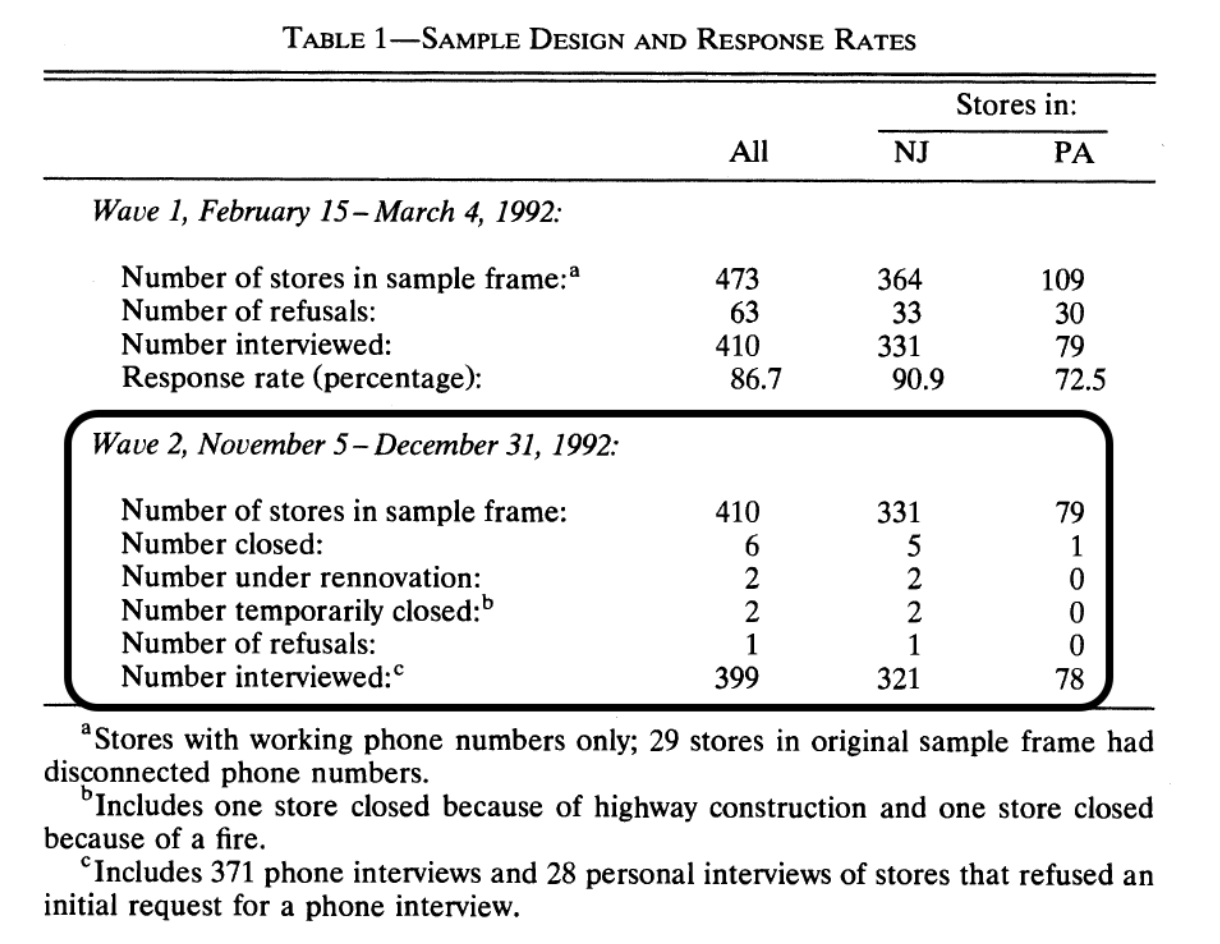
\includegraphics[width=0.63\textwidth]{figures/CardKrueger_Table1.png}
  \caption{Table 1 from Card and Krueger (1994).}
  \label{fig:CK_Tab1}
\end{table}

\begin{table}[!htb]
\centering
  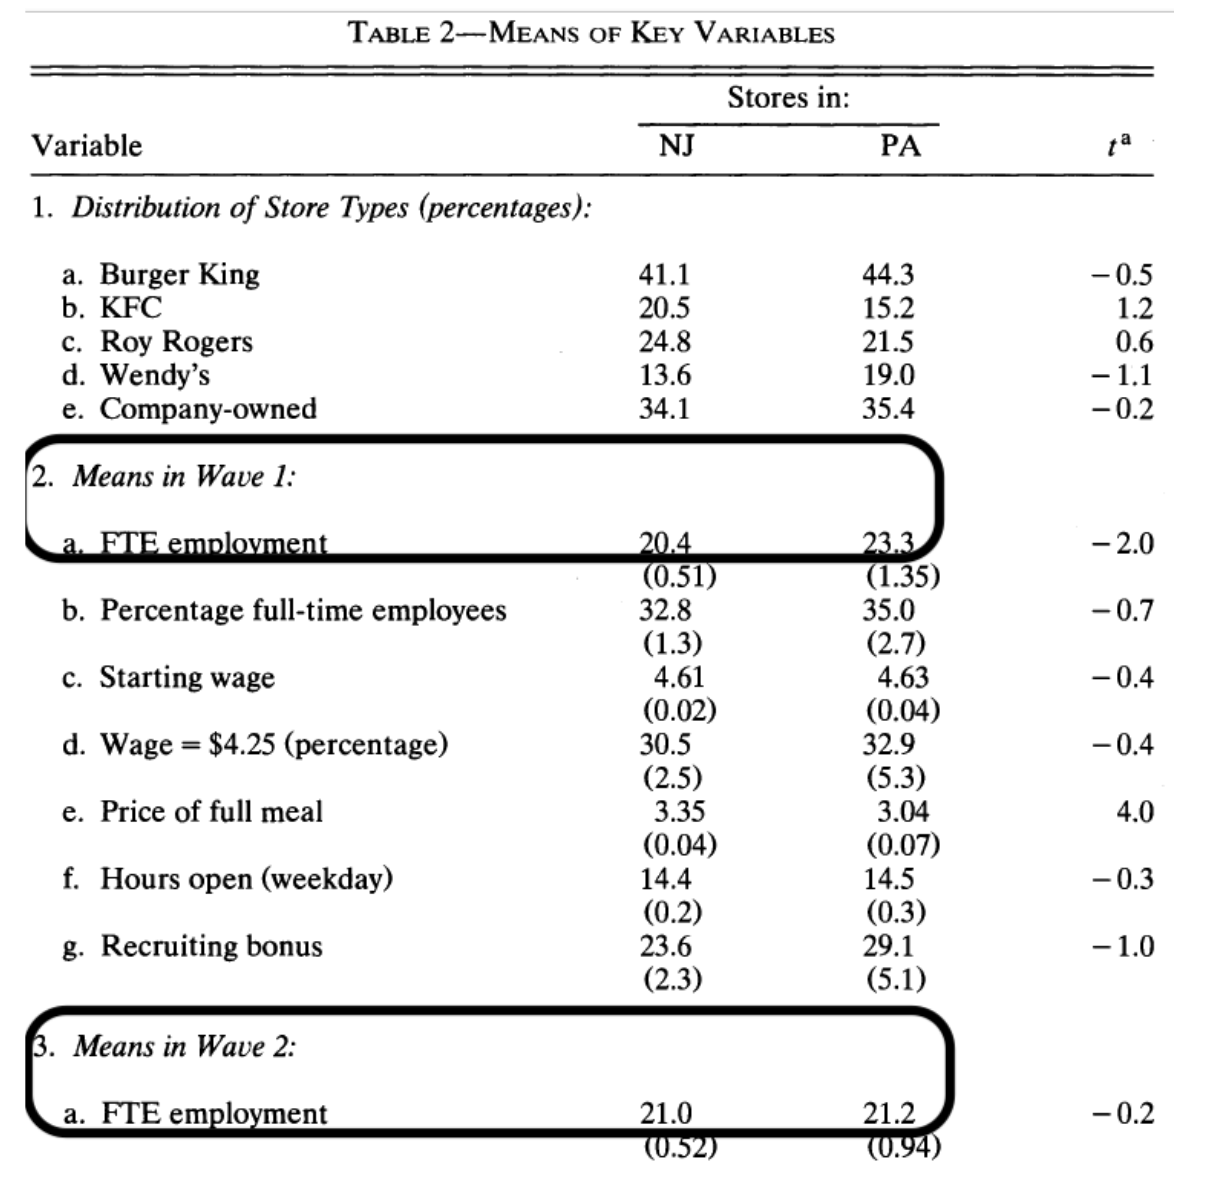
\includegraphics[width=0.63\textwidth]{figures/CardKrueger_Table2.png}
  \caption{Table 2 from Card and Krueger (1994).}
  \label{fig:CK_Tab2}
\end{table}

\newpage
\begin{table}[!htb]
\centering
  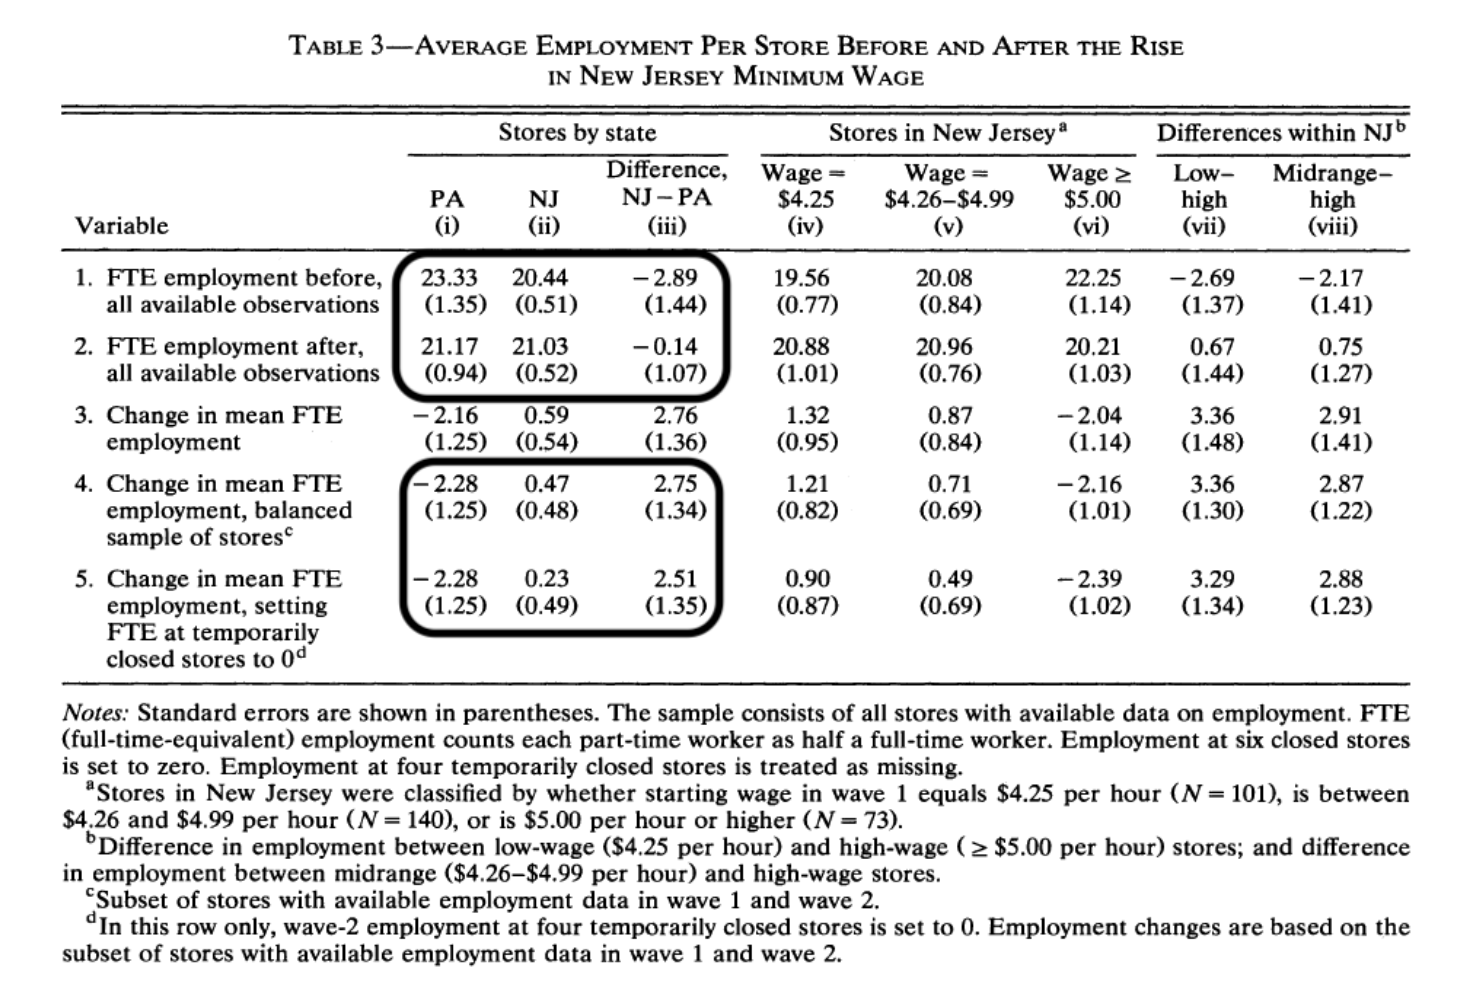
\includegraphics[width=0.75\textwidth]{figures/CardKrueger_Table3.png}
  \caption{Table 3 from Card and Krueger (1994).}
  \label{fig:CK_Tab3}
\end{table}

\begin{table}[!htb]
\centering
  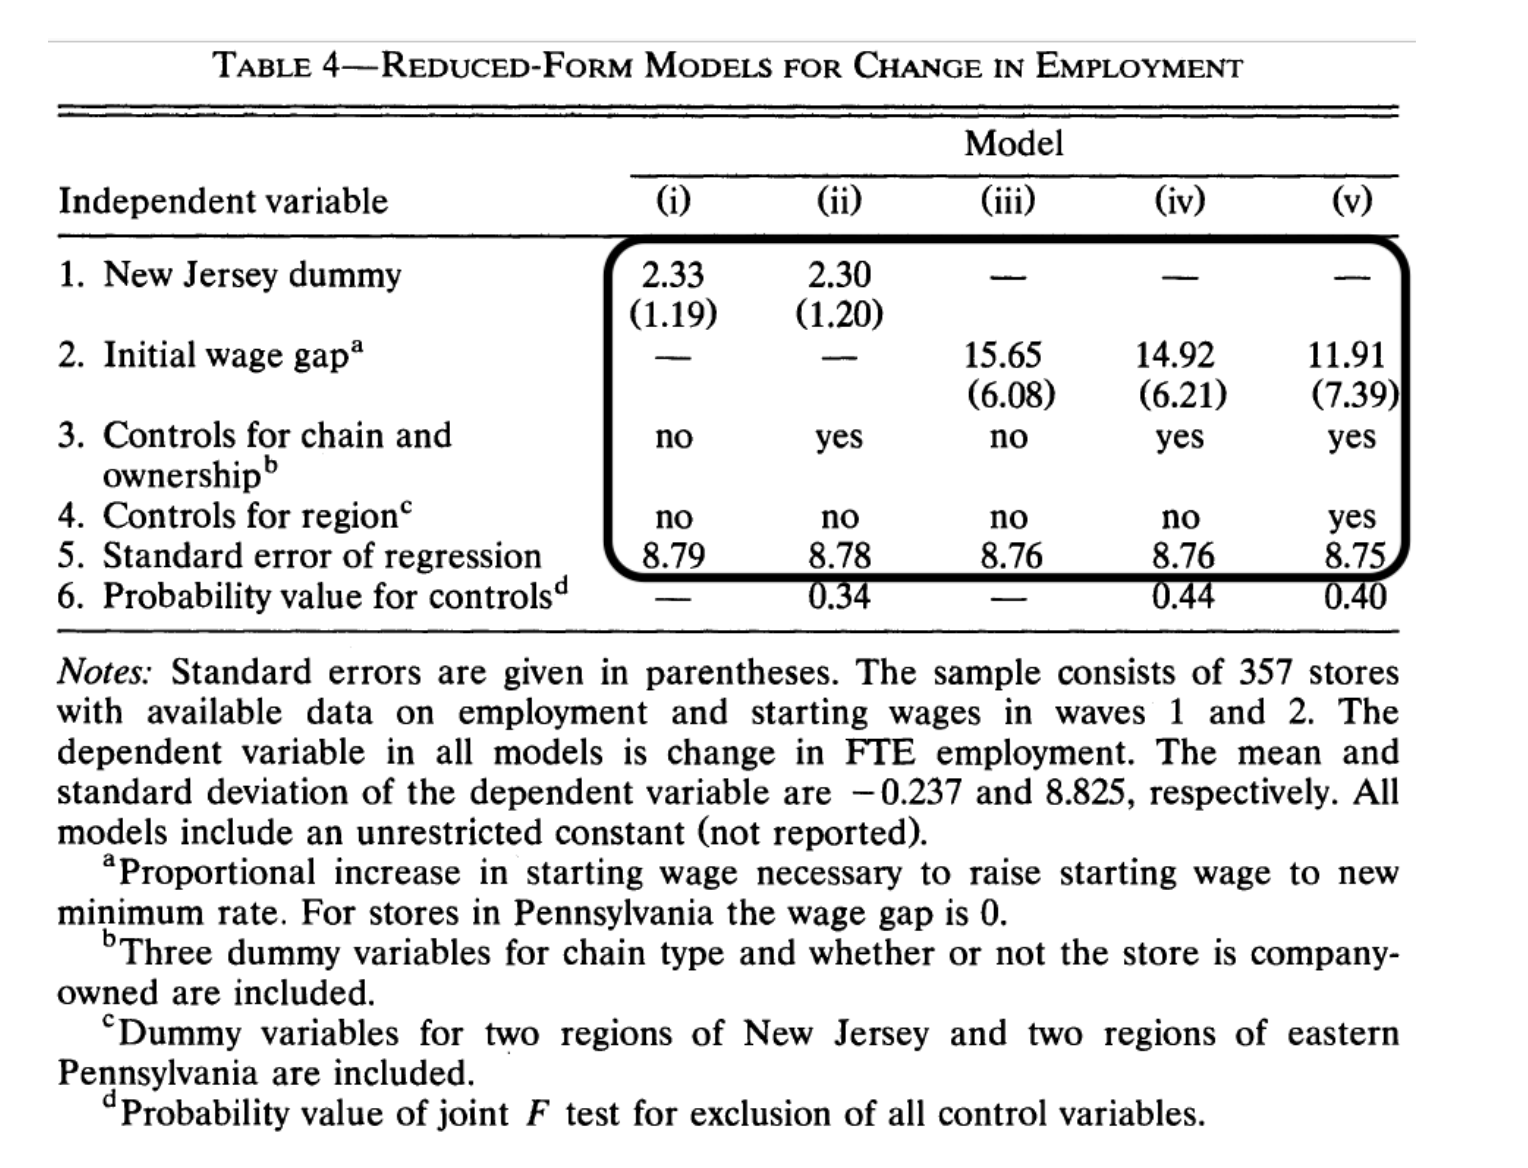
\includegraphics[width=0.75\textwidth]{figures/CardKrueger_Table4.png}
  \caption{Table 4 from Card and Krueger (1994).}
  \label{fig:CK_Tab4}
\end{table}

\end{document}
